% =====================================================================
%  Chapitre 2 -- Le RNN
%  Partie b : formes d'entree/sortie, seq2seq, quiz, TP2
% =====================================================================

\begin{frame}{Une même cellule, plusieurs usages}
\begin{center}
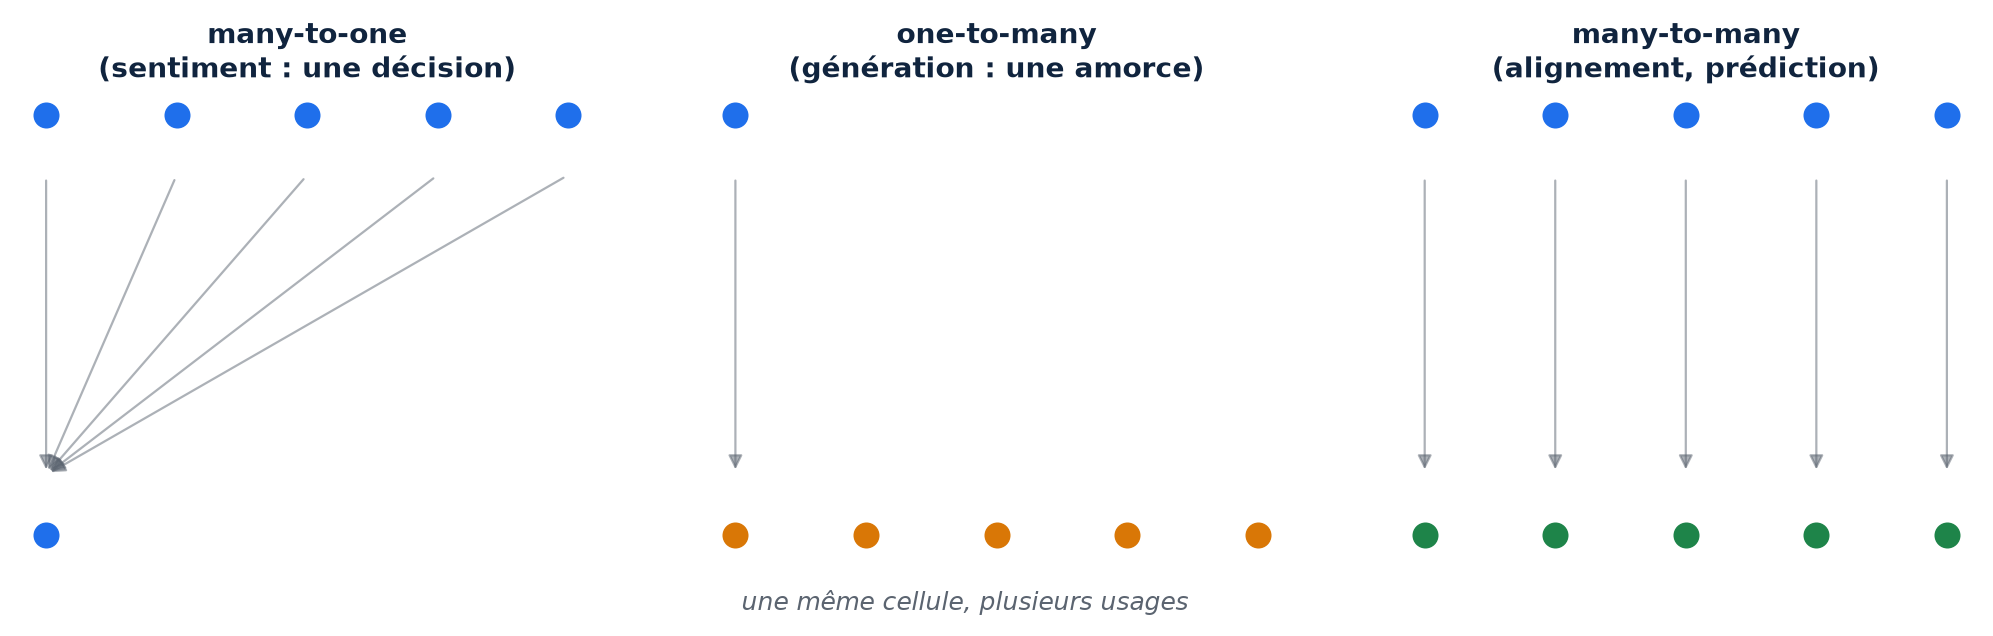
\includegraphics[width=0.95\textwidth]{s07_formes_es.png}
\end{center}
\vspace{1mm}
\begin{columns}[t]
\begin{column}{0.32\textwidth}
\begin{ebox}[many-to-one]
Lire toute une critique, décider une fois : \textbf{sentiment}.
\end{ebox}
\end{column}
\begin{column}{0.32\textwidth}
\begin{ebox}[one-to-many]
Une amorce, puis générer une suite : \textbf{texte}.
\end{ebox}
\end{column}
\begin{column}{0.32\textwidth}
\begin{ebox}[many-to-many]
Un pas, une sortie : \textbf{étiquetage}, prédiction pas à pas.
\end{ebox}
\end{column}
\end{columns}
\end{frame}

\begin{frame}{Seq2seq : traduire, résumer, transcrire}
\begin{center}
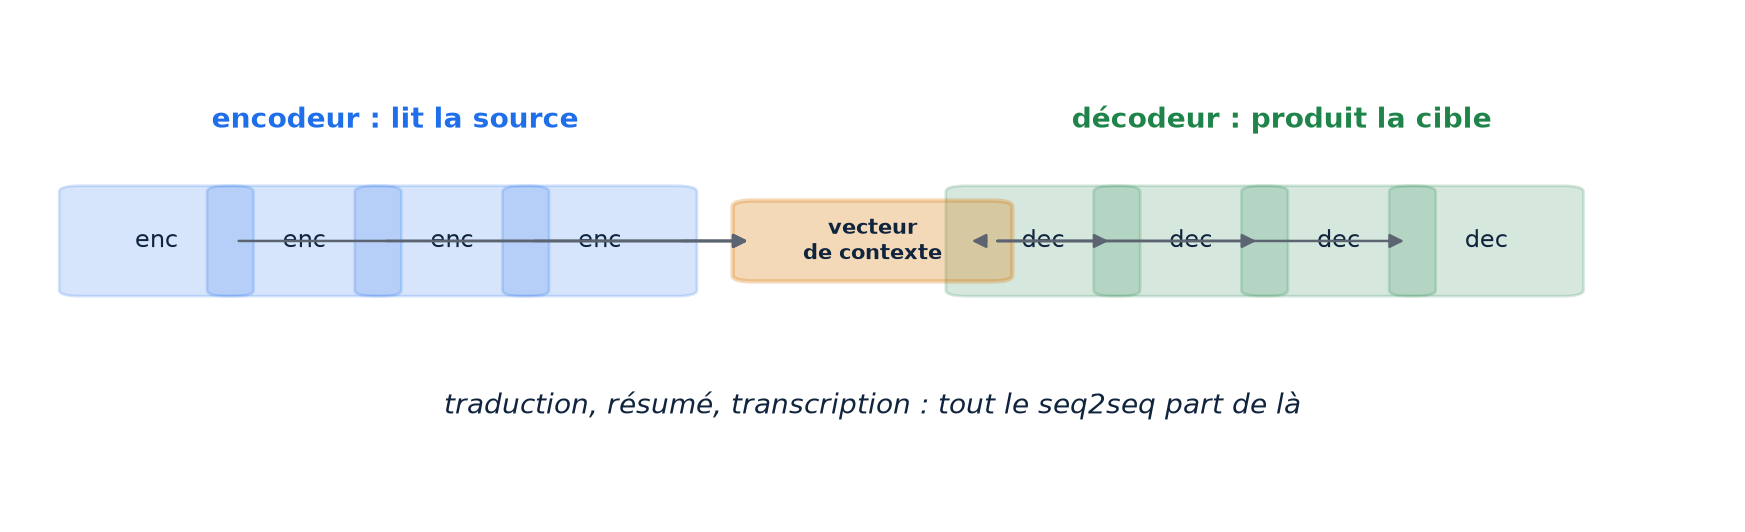
\includegraphics[width=0.9\textwidth]{s08_seq2seq.png}
\end{center}
\vspace{1mm}
\begin{itemize}
  \item L'\textbf{encodeur} lit la source et condense tout dans un vecteur
  de contexte.
  \item Le \textbf{décodeur} produit la cible à partir de ce vecteur.
\end{itemize}
\begin{wbox}[Le goulot d'étranglement]
Tout le contenu de la source passe par un vecteur unique : pour les longues
séquences, c'est insuffisant --- d'où l'attention (chapitre 3).
\end{wbox}
\end{frame}

\begin{frame}[fragile]{Seq2seq en pratique : le décodeur génère mot à mot}
\begin{columns}[t]
\begin{column}{0.52\textwidth}
\begin{itemize}
  \item À chaque pas, le décodeur produit une \textbf{distribution}
  sur le vocabulaire (softmax).
  \item On choisit le mot le plus probable --- ou l'on échantillonne
  (chapitre 4).
  \item Ce mot devient l'entrée du pas suivant.
\end{itemize}
\end{column}
\begin{column}{0.44\textwidth}
\begin{codebox}[Boucle de génération]
\begin{lstlisting}
h = contexte
mot = "<debut>"
while mot != "<fin>":
    logits = decodeur(mot, h)
    mot = vocab[int(logits.argmax())]
    sortie.append(mot)
\end{lstlisting}
\end{codebox}
\end{column}
\end{columns}
\end{frame}

\begin{frame}{Quiz 2 --- le RNN}
\begin{qbox}[Question 1]
Le nombre de paramètres d'une couche RNN dépend-il de la longueur $T$ des séquences ?
\begin{itemize}
  \item[(a)] oui, linéairement \quad (b) non, jamais \quad (c) oui, en $T^2$
\end{itemize}
\end{qbox}
\begin{qbox}[Question 2]
Avec un rayon spectral $r = 0{,}55$, combien reste-t-il du gradient après 20 pas ?
\begin{itemize}
  \item[(a)] $\approx 0{,}55$ \quad (b) $\approx 6 \times 10^{-6}$
  \quad (c) $\approx 406$
\end{itemize}
\end{qbox}
\begin{qbox}[Question 3]
Le clipping de gradient traite…
\begin{itemize}
  \item[(a)] l'évanouissement \quad (b) l'explosion \quad (c) les deux
\end{itemize}
\end{qbox}
\begin{qbox}[Question 4]
Classer une critique en positive/négative est une tâche…
\begin{itemize}
  \item[(a)] one-to-many \quad (b) many-to-one \quad (c) many-to-many
\end{itemize}
\end{qbox}

% [fix] bloc deplace
\end{frame}
\begin{frame}{Quiz 2 --- le RNN (suite)}
\begin{solbox}[Réponses]
\textbf{1.} (b) : le partage de poids est total. \quad
\textbf{2.} (b) : $0{,}55^{20} = 6{,}4 \cdot 10^{-6}$. \quad
\textbf{3.} (b) : on borne la norme. \quad
\textbf{4.} (b) : toute la séquence, une seule décision.
\end{solbox}
\end{frame}

\begin{frame}{À retenir et TP}
\begin{kbox}[Les trois idées du chapitre 2]
\begin{enumerate}
  \item Une \textbf{cellule unique} déroulée dans le temps : mêmes poids
  à chaque pas, état caché transmis.
  \item $h_t = \tanh(W_x x_t + W_h h_{t-1} + b)$ --- tout est là.
  \item Le gradient le long du temps est un \textbf{produit} : évanescence
  ou explosion, selon le rayon spectral.
\end{enumerate}
\end{kbox}
\vspace{1.5mm}
\begin{abox}[TP2 : \file{notebooks/TP2_RNN_serie_temporelle.ipynb}]
Coder la cellule à la main, vérifier l'évanouissement du gradient, puis entraîner
un RNN à prédire la suite d'une série. Durée : \textbf{2 h} · barème : \textbf{10 points}.
\end{abox}
\end{frame}
